%!TEX root = /Users/Daniel/Documents/Imperial/project/tevatron-higgs/report/report.tex

In any scenario where statistical methods are used to interpret data selecting features in order to maximise the discriminatory or explanatory power of the model plays a critical role.
From the b-tagged jets, the jets with the highest and second highest transverse momentum $P_t$ were identified as being the putative product of the decaying Higgs boson, with all the following variable differences are considered to be taken between these leading jets. 
From the raw simulation data, following \cite{Abazov201197} seven feature variables were extracted and used as inputs to the classification neural network. 

\subsubsection*{Pseudorapidity difference $ \Delta\eta $ } % (fold)
\label{ssub:pseudorapidity}

Te pseudorapidity of a jet is defined as
\begin{equation}
	\eta = - \ln\left[\tan\left( \frac{\theta}{2} \right)\right]
\end{equation}
where $\theta$ is the angle between the jet and the beam axis. The pseudorapidity is preferred to the $\theta$ as it is Lorentz invariant.
% subsubsection pseudorapidity (end)


\subsubsection*{Momentum balance $P_{balance}$} % (fold)
\label{ssub:momentum_balance_p__balance}

The momentum balance of the leading b jet pair is defined

\begin{equation}
	P_{balance} = \frac{\left|p_1 - p_2\right|}{ \left|p_1 + p_2\right|}  
\end{equation}

% subsubsection momentum_balance_p__balance (end)

\subsubsection*{Sphericity $S$} % (fold)
\label{ssub:sphericity_s}
	The sphericity is defined as 
	\begin{equation}
		S = \frac{3}{2} (\lambda_2 + \lambda_3)
	\end{equation}

	where $\lambda_2$ and $\lambda_3$ are the second and third largest eigenvalues of the sphericity tensor $\mathbf{\hat{S}}^{\alpha\beta}$
	\begin{equation}
		\mathbf{\hat{S}}^{\alpha\beta} = \frac{\sum_i p_{\alpha}^i p_{\beta}^i}{\sum_i |p^i|^2}
	\end{equation}

% subsubsection sphericity_s (end)


Additionally we define the \textbf{azimuthal angle difference $ \Delta\phi $}, the \textbf{combined pseudorapidity $\eta_H$}, the \textbf{difference between the leading jet and the Higgs $\eta_H - \eta_1$} and the \textbf{invariant di-jet mass $M_H$}.




\begin{figure}[htbp]
	\centering	
	\begin{subfigure}[b]{0.25\textwidth}
	                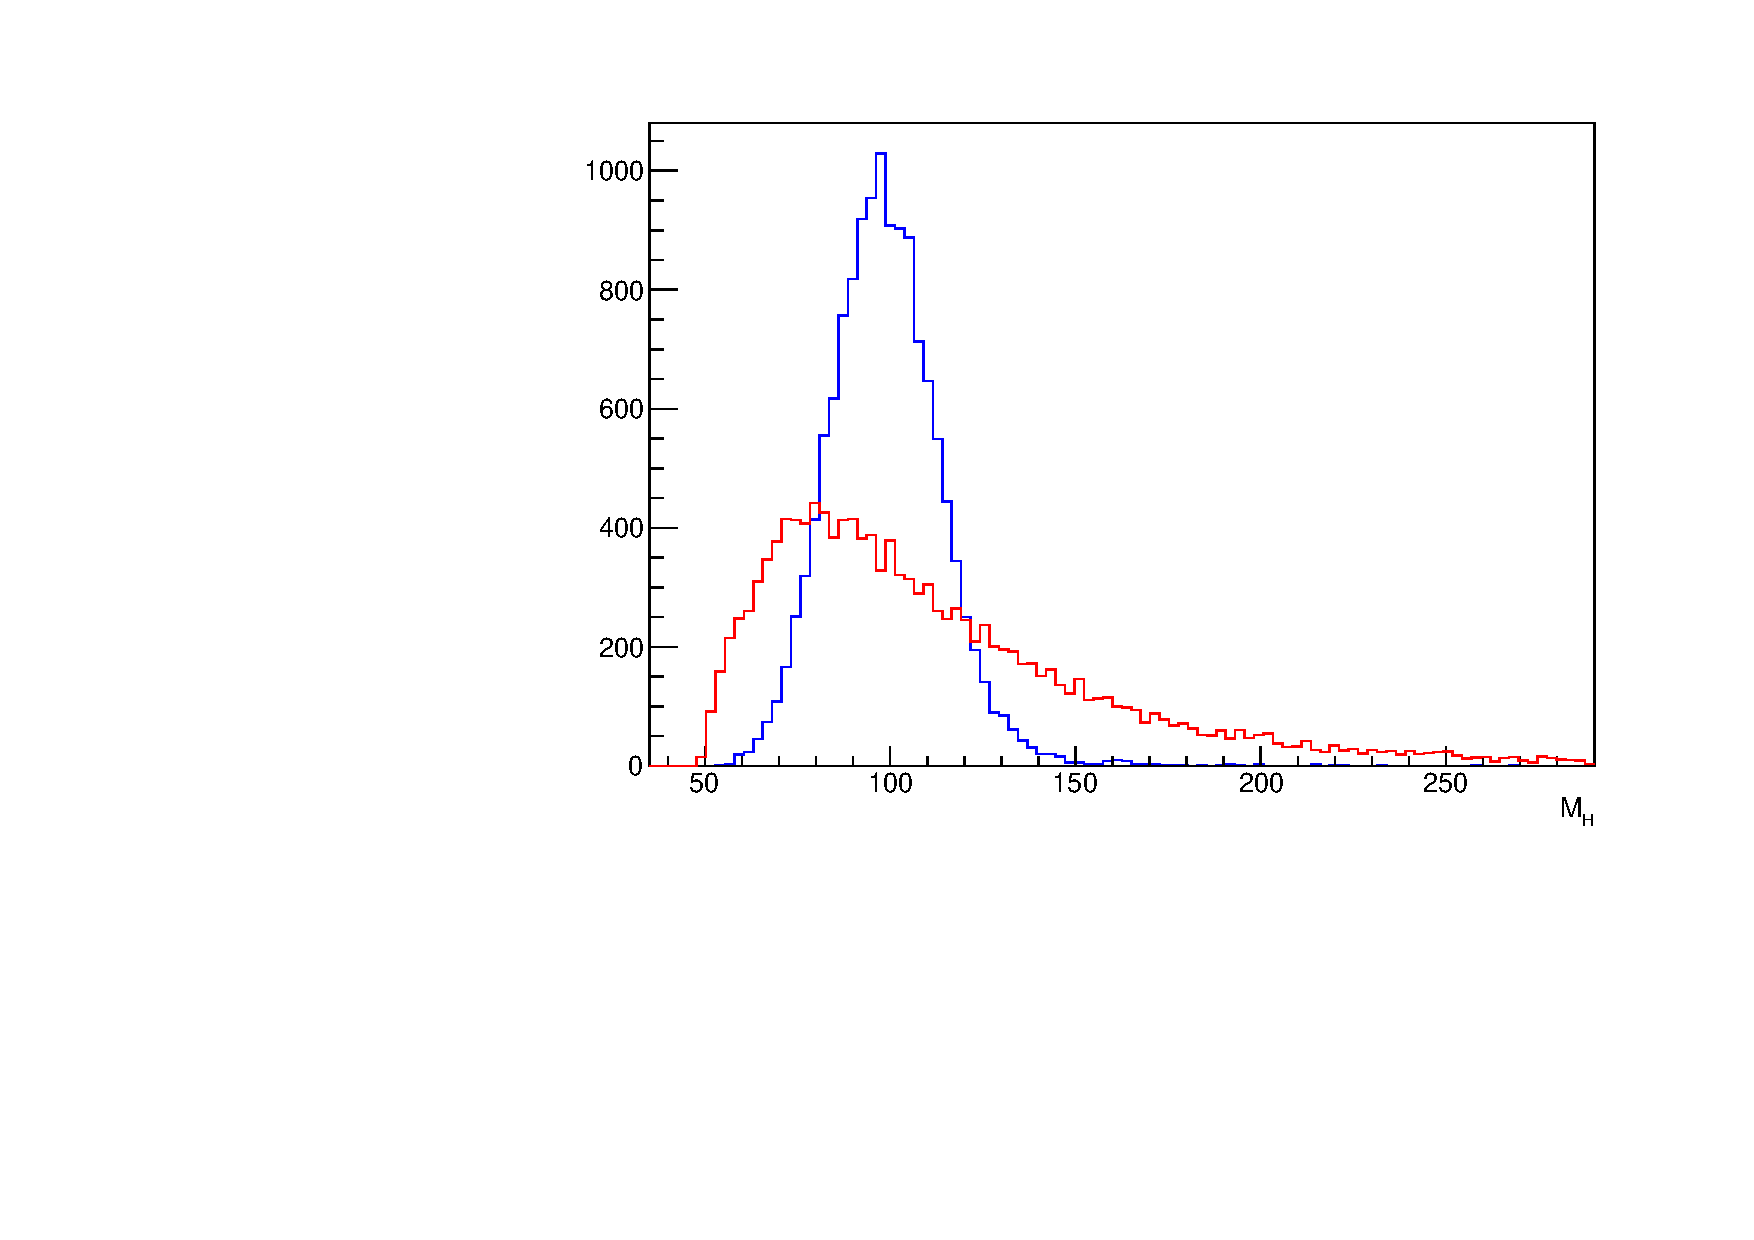
\includegraphics[width=\textwidth]{img/mh}
	                \caption{Invariant mass}
	                \label{fig:mh}
	\end{subfigure}
	\begin{subfigure}[b]{0.25\textwidth}
	                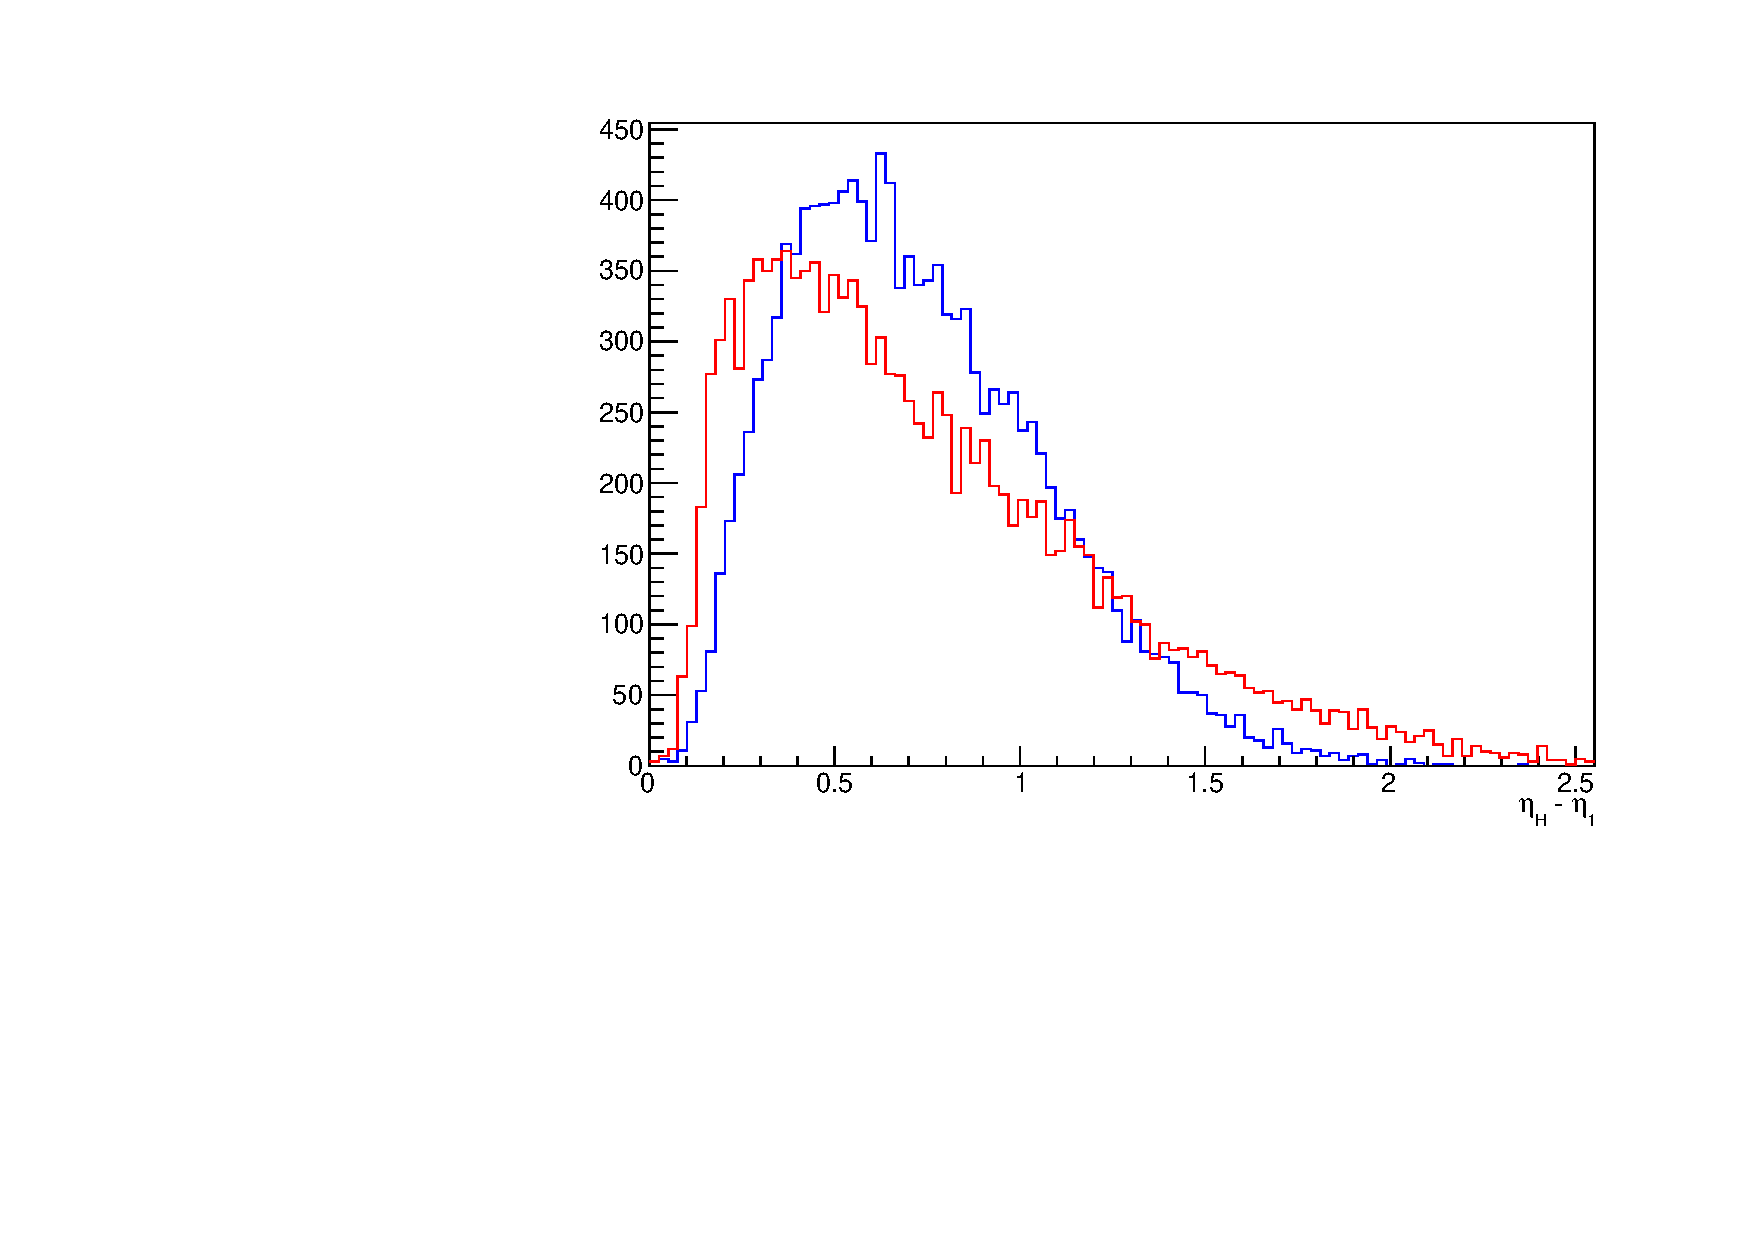
\includegraphics[width=\textwidth]{img/angle}
	                \caption{$\eta_H - \eta_1$}
	                \label{fig:angle}
	\end{subfigure}
	\begin{subfigure}[b]{0.25\textwidth}
	                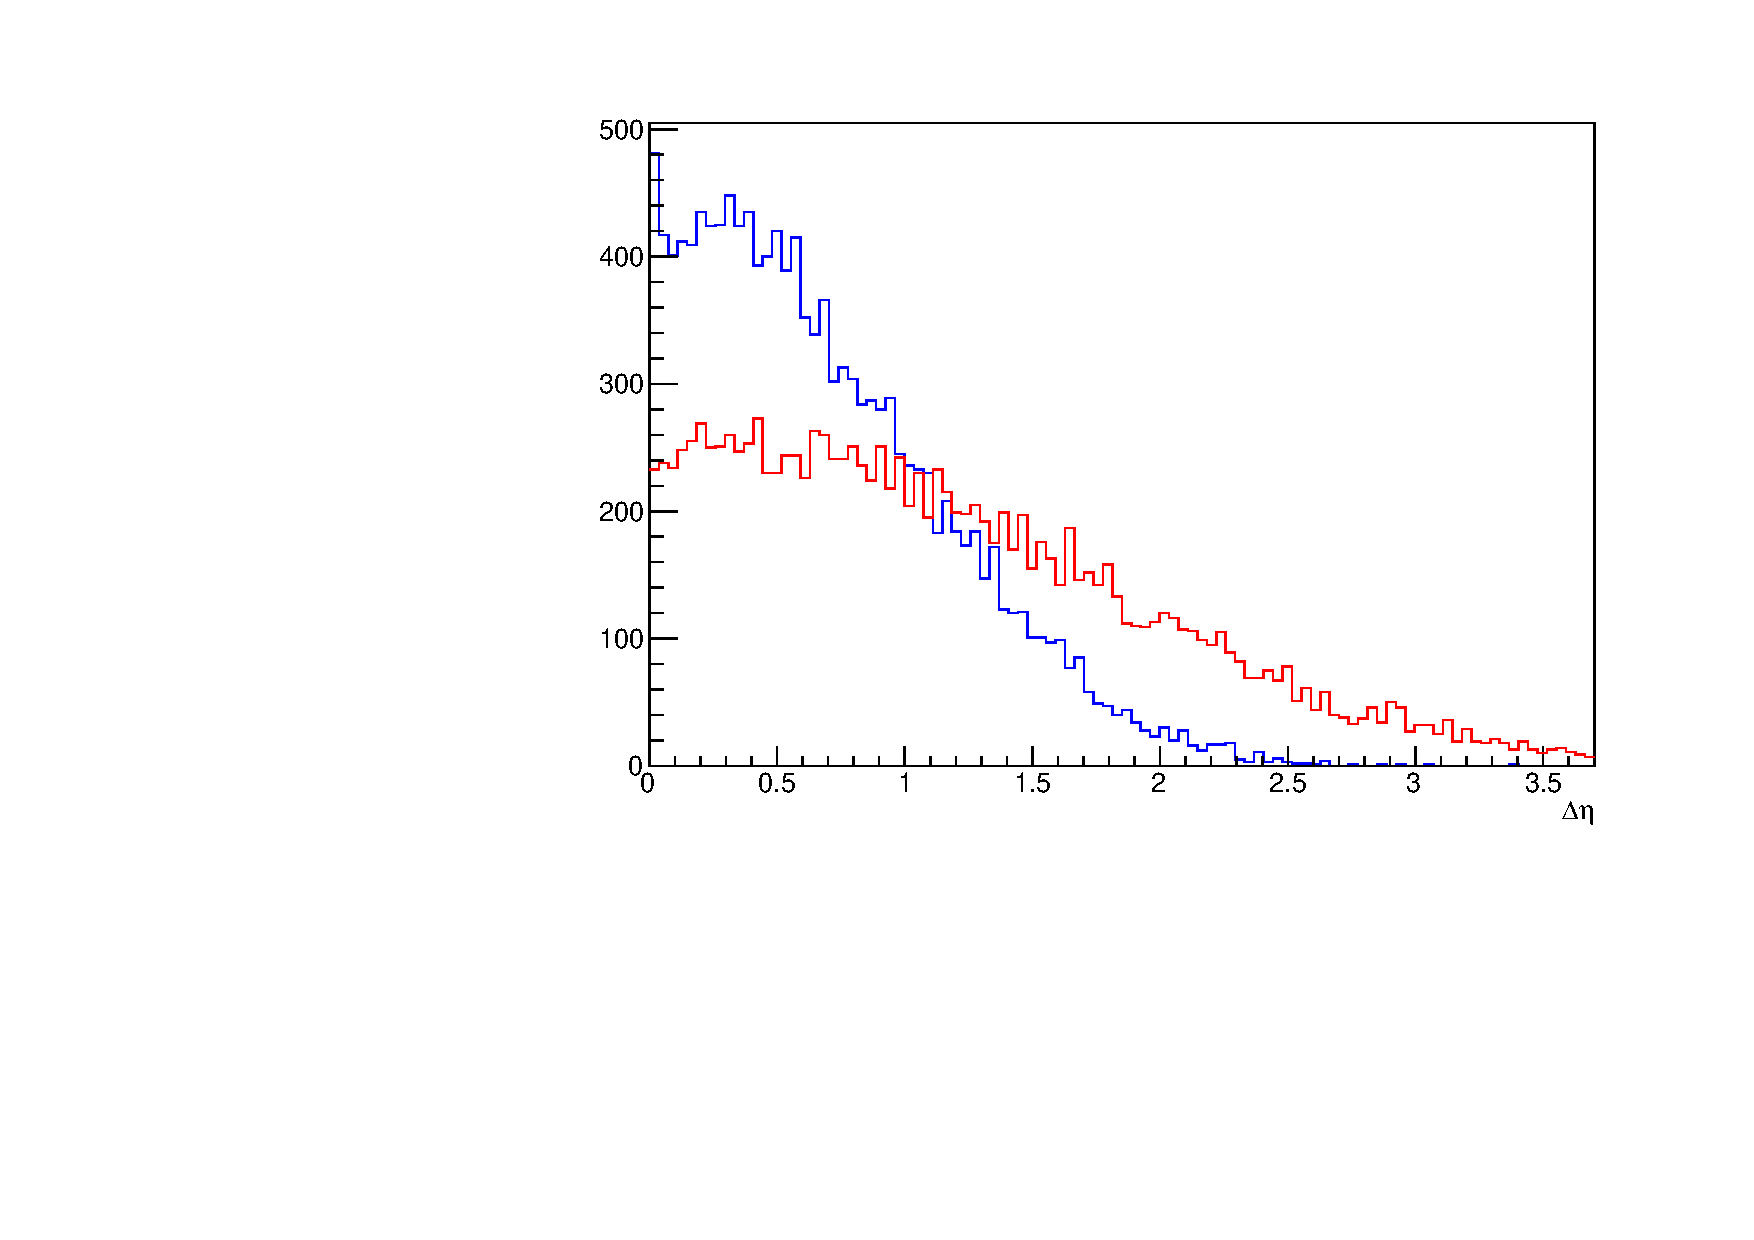
\includegraphics[width=\textwidth]{img/deta}
	                \caption{$\Delta\eta$}
	                \label{fig:deta}
	\end{subfigure}
	\begin{subfigure}[b]{0.25\textwidth}
	                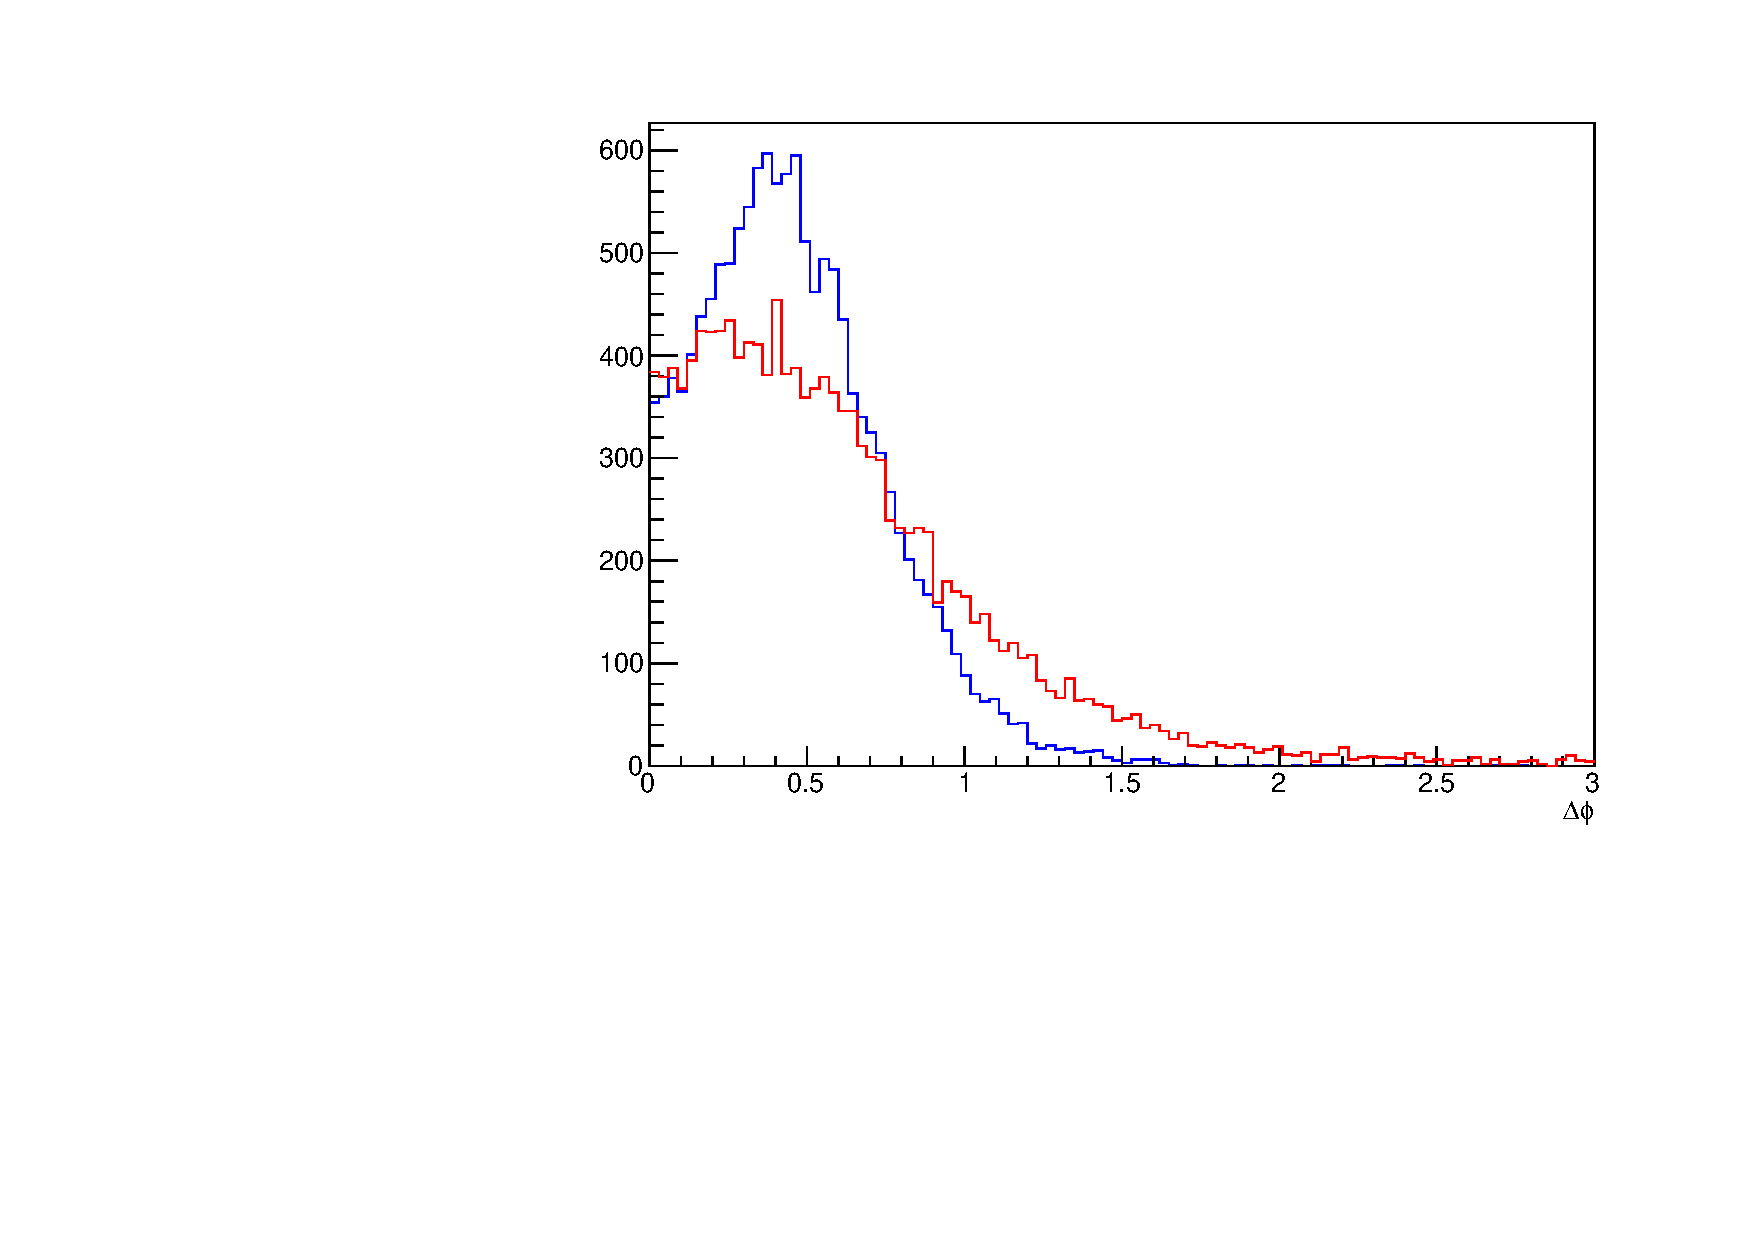
\includegraphics[width=\textwidth]{img/dphi}
	                \caption{$\Delta\phi$}
	                \label{fig:dphi}
	\end{subfigure}	
	\begin{subfigure}[b]{0.25\textwidth}
	                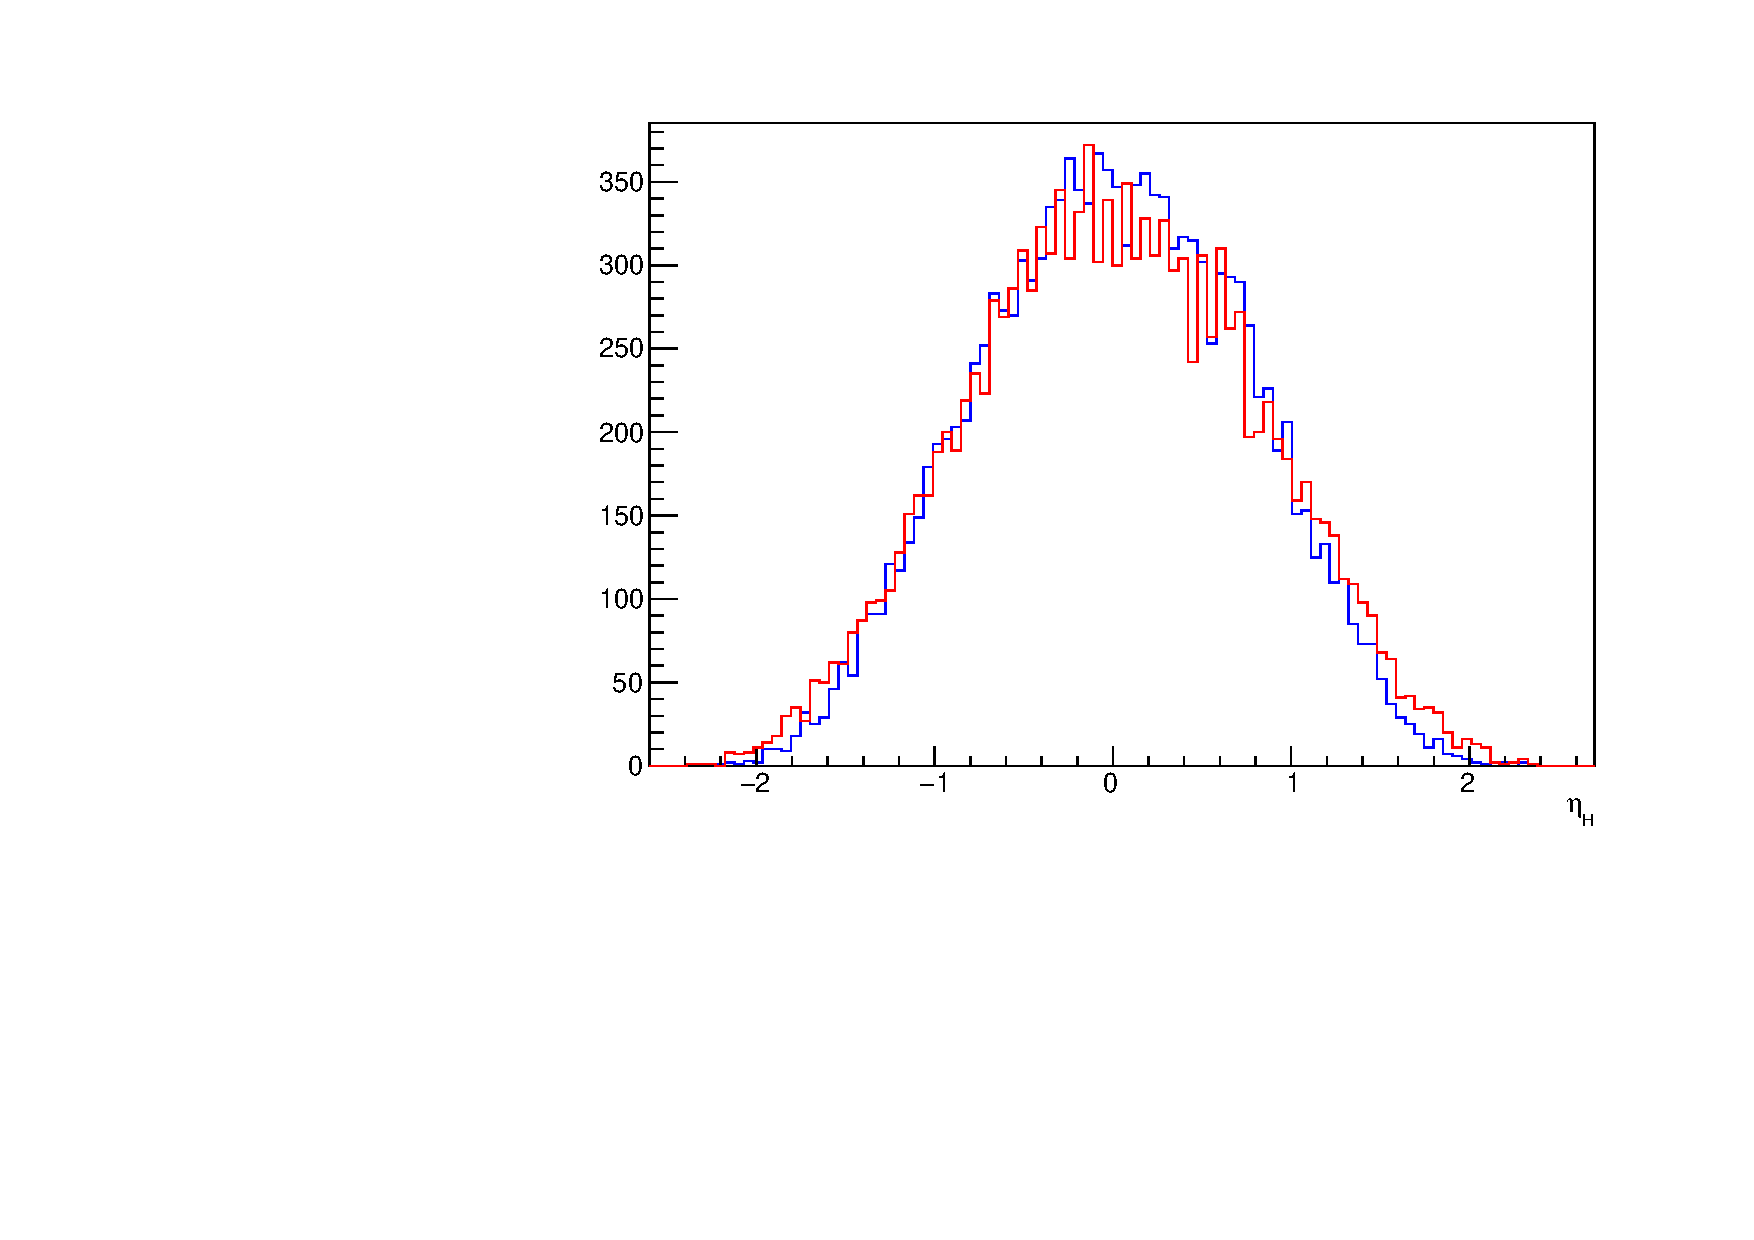
\includegraphics[width=\textwidth]{img/etah}
	                \caption{$\eta_H$}
	                \label{fig:etah}
	\end{subfigure}
	\begin{subfigure}[b]{0.25\textwidth}
	                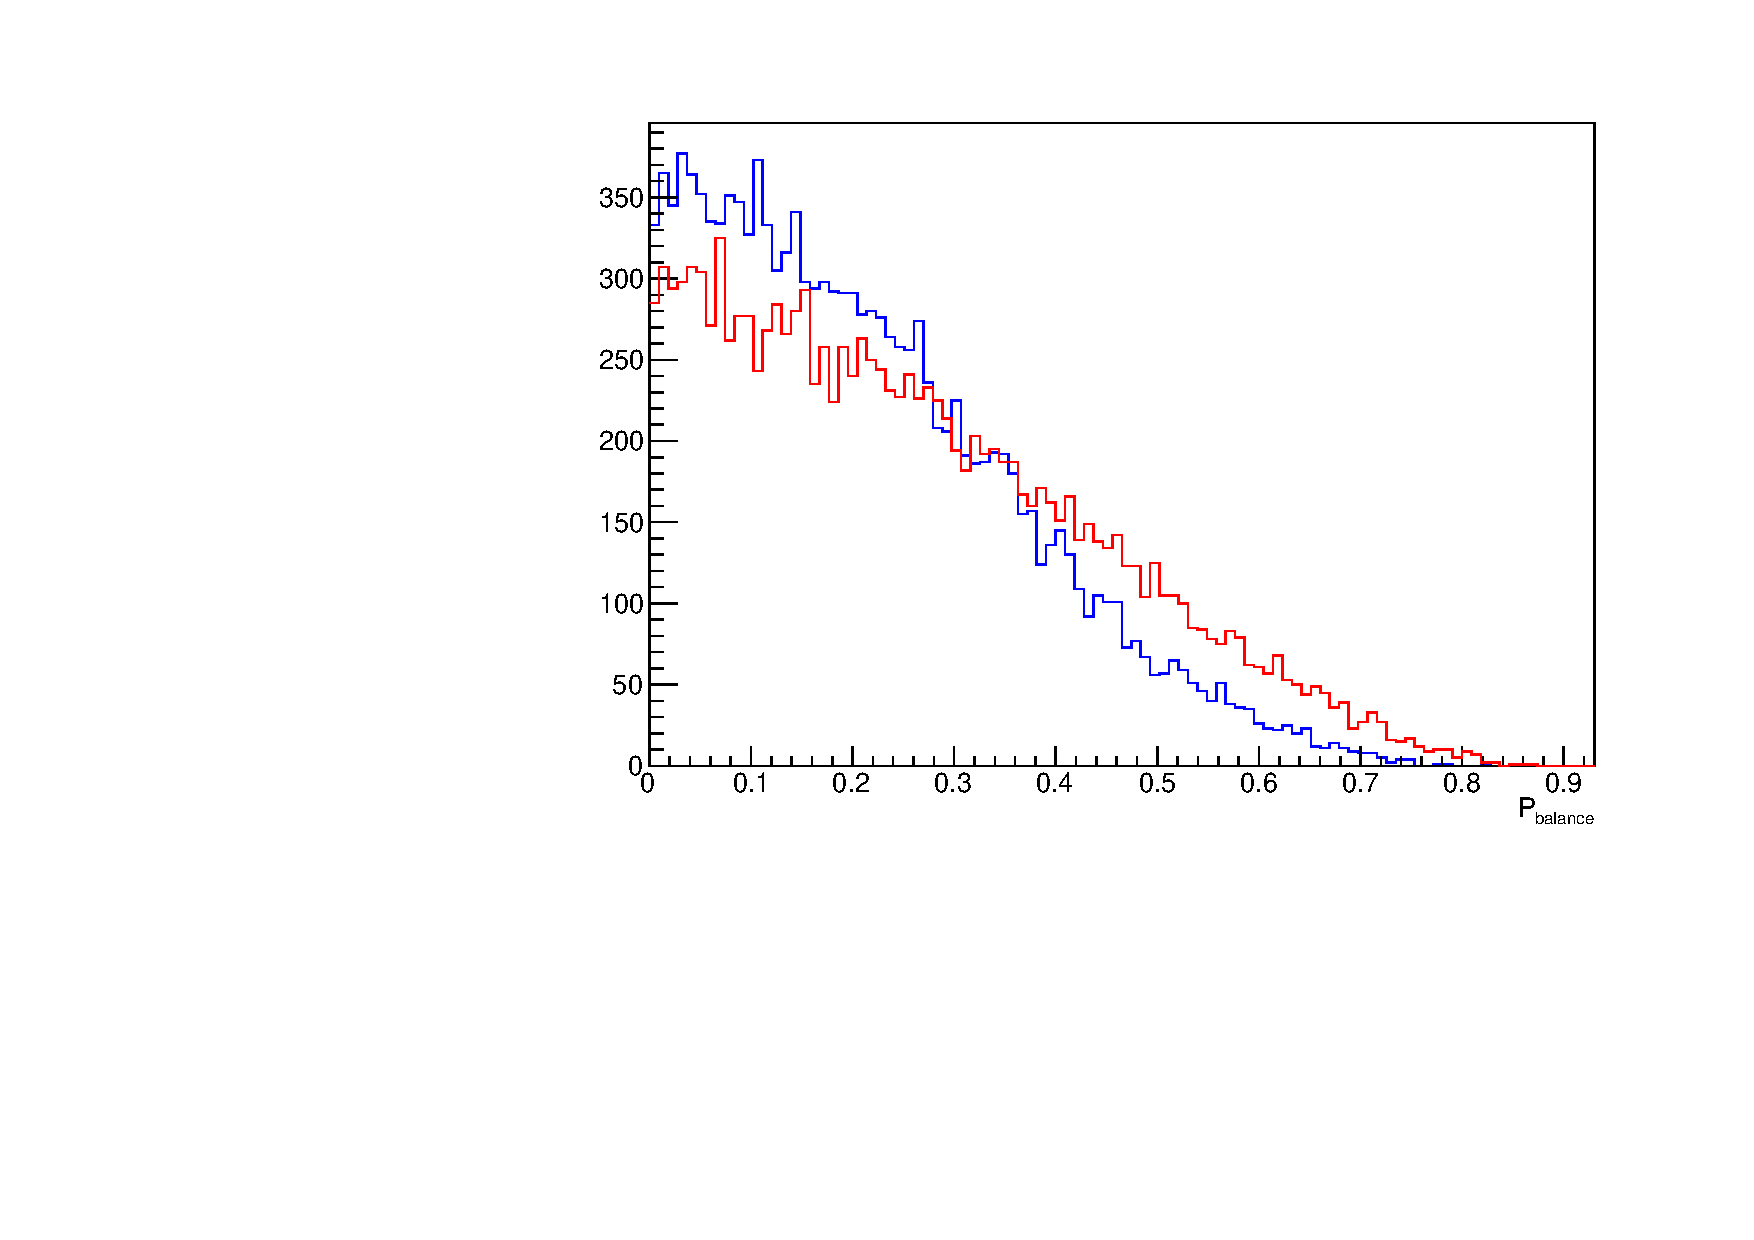
\includegraphics[width=\textwidth]{img/pbalance}
	                \caption{Momentum balance}
	                \label{fig:pbal}
	\end{subfigure}
	\begin{subfigure}[b]{0.25\textwidth}
	                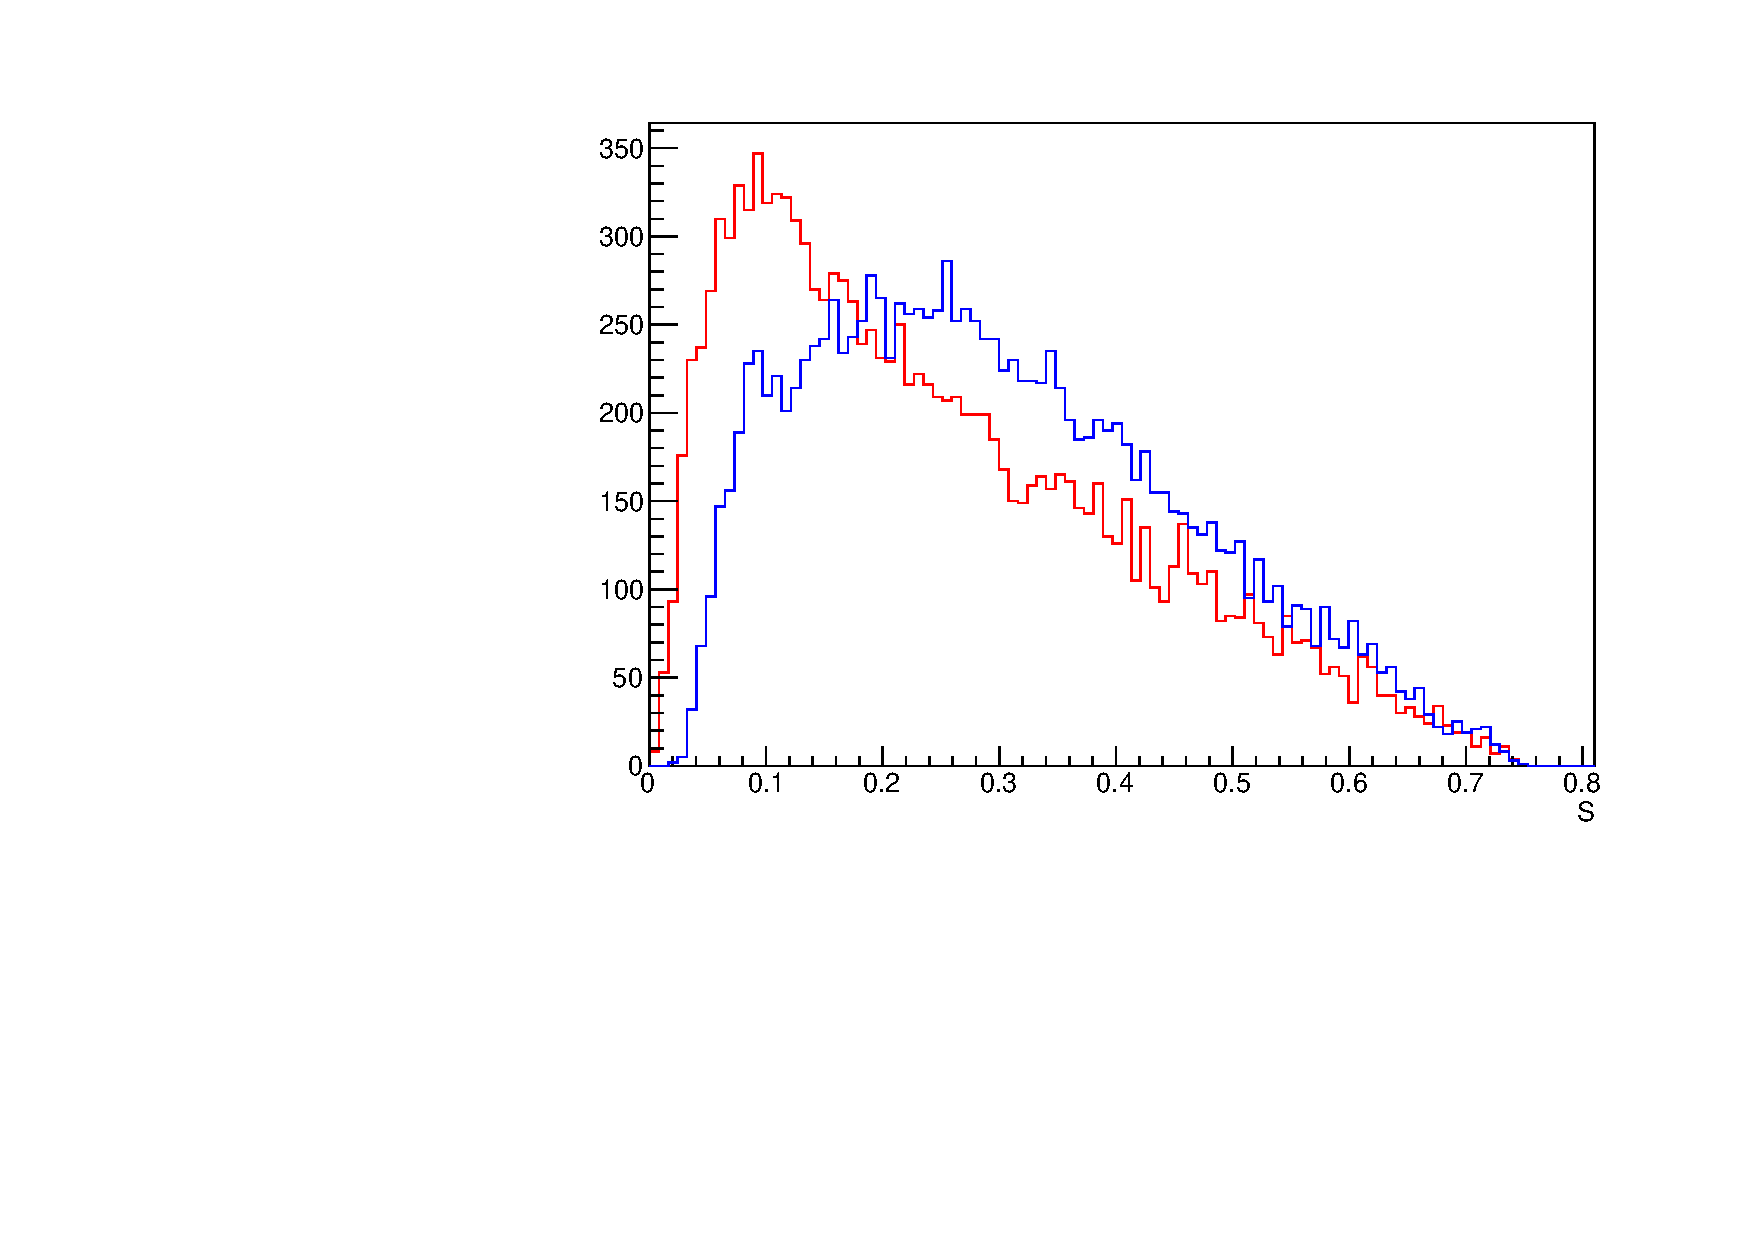
\includegraphics[width=\textwidth]{img/sphericity}
	                \caption{Sphericity}
	                \label{fig:sphericity}
	\end{subfigure}

	\caption{Distributions of the input features. All y scales are events. The signal is in blue and the background in red.}
	
	\label{fig:label}
\end{figure} 

